\subsection{3 Sites Results}

We will look at several metrics: waiting time, overtime and number
of diverted volunteers. The reason why we want to look at number of
diverted volunteers is that diversion involves communication and
coordination with patients, so we'd like to achieve improvement
without too much change.

\begin{figure}[htp]
\centering
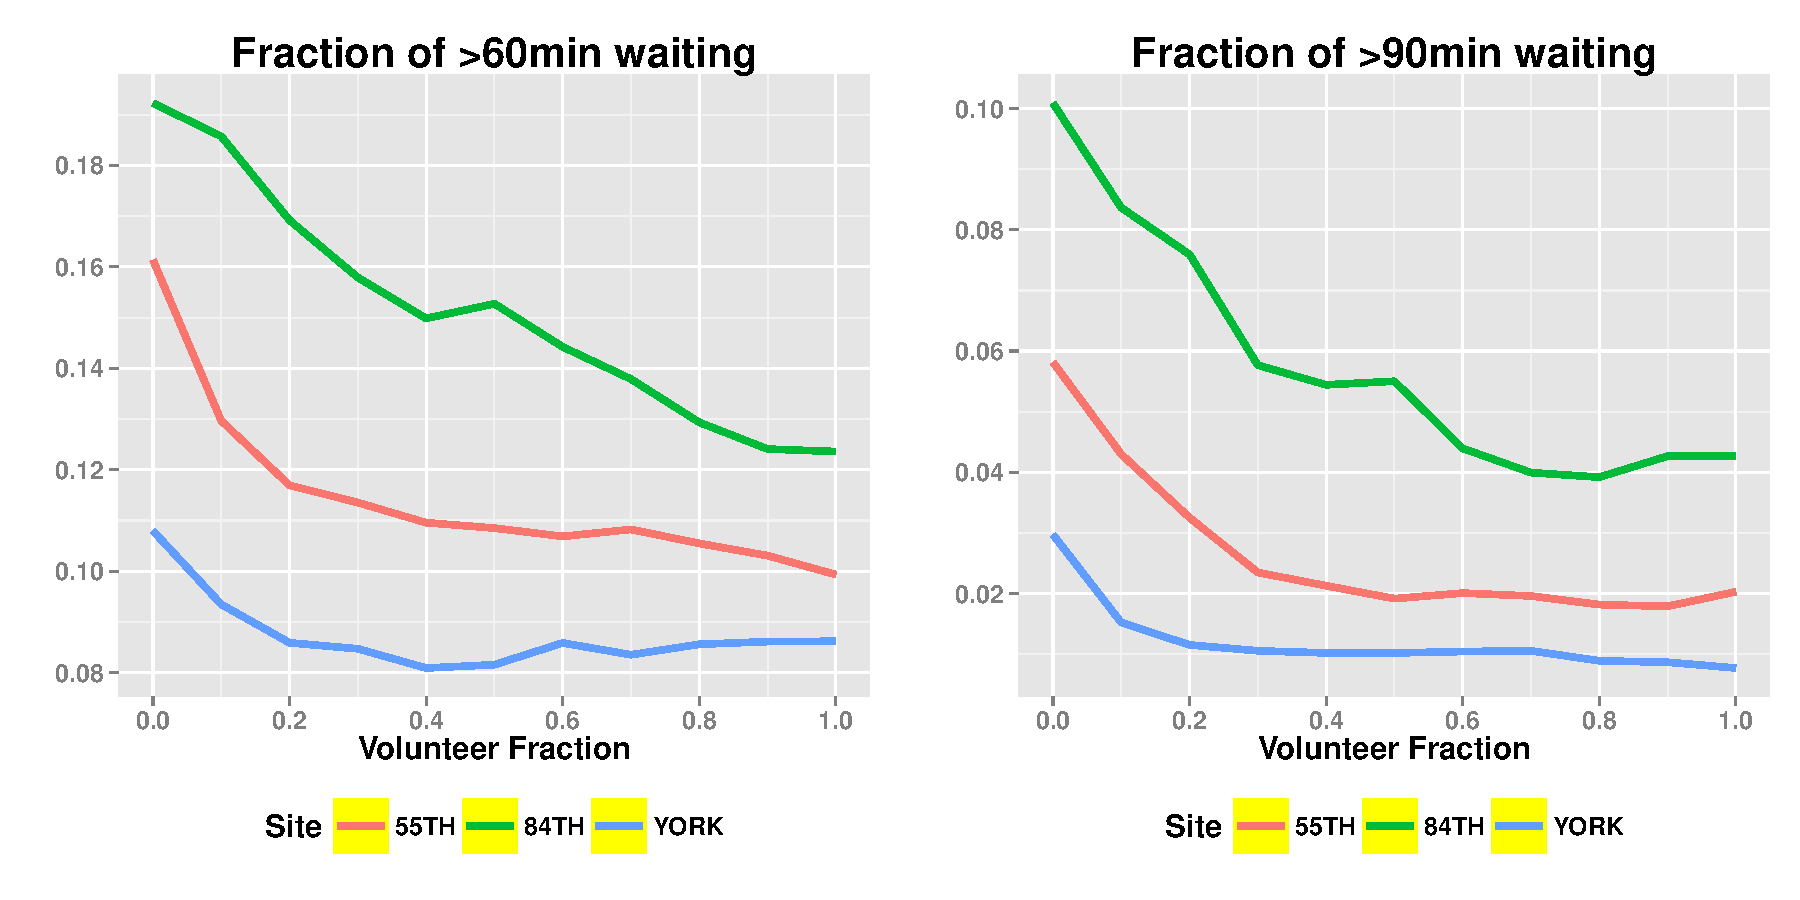
\includegraphics[width=.9\textwidth]{chap3/numeric/pic/3sites_extreme}
\caption{The impact on extreme waiting by diversions. As we increase
fraction of volunteers, we have more flexibility to divert patients,
and we see the extreme waiting cases drop.}
\label{fig:3sites_extreme}
\end{figure}

Figure \ref{fig:3sites_extreme} show how diversion affects extreme waiting times. Without
diversion, about 13.5\% patients wait more than 60min and about
5\% patients wait more than 90min. When we have 40\% patients
as volunteers and 60min lead time, only 10\% patients wait more
than 60min and 2\% patients wait more than 90min.

\begin{figure}[htp]
\centering
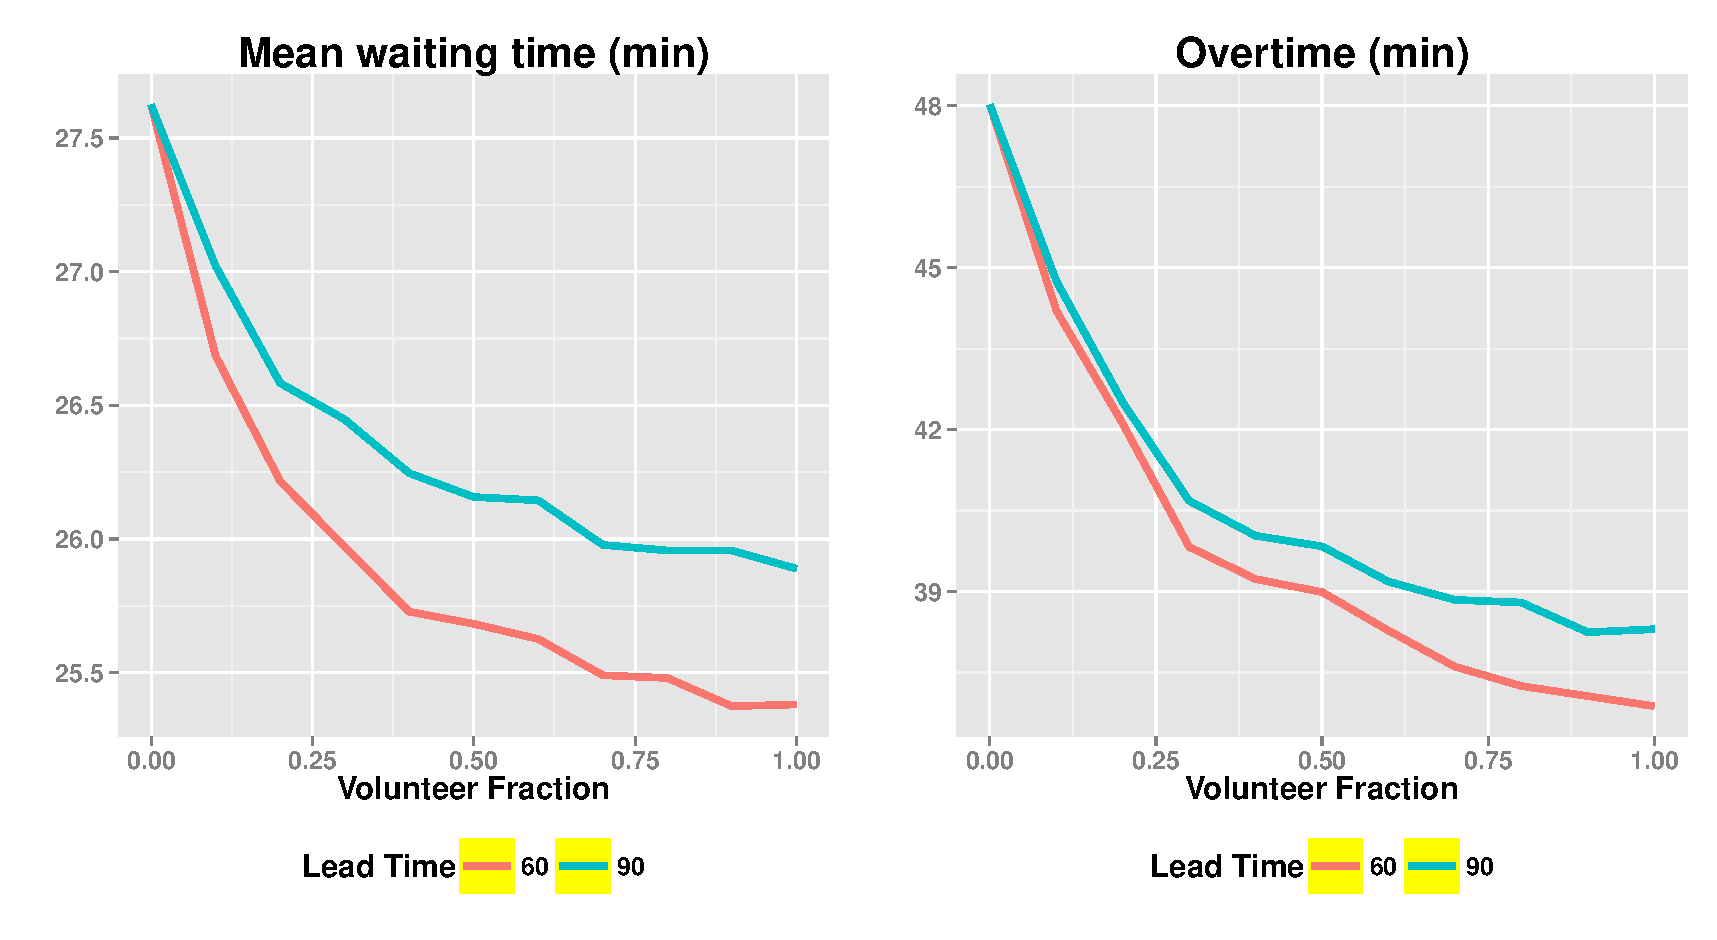
\includegraphics[width=.9\textwidth]{chap3/numeric/pic/3sites_wait_overtime}
\caption{The impact of diversions on mean waiting time and
sites overtime. There is mild improvement on both metric.}
\label{fig:3sites_wait_overtime}
\end{figure}

Figure \ref{fig:3sites_wait_overtime} shows
that we also have mild improvement over mean waiting time of all
patients. Figure \ref{fig:3sites_wait_overtime} shows that with diversion, we also reduce
mean overtime over all sites.

\begin{figure}[htp]
\centering
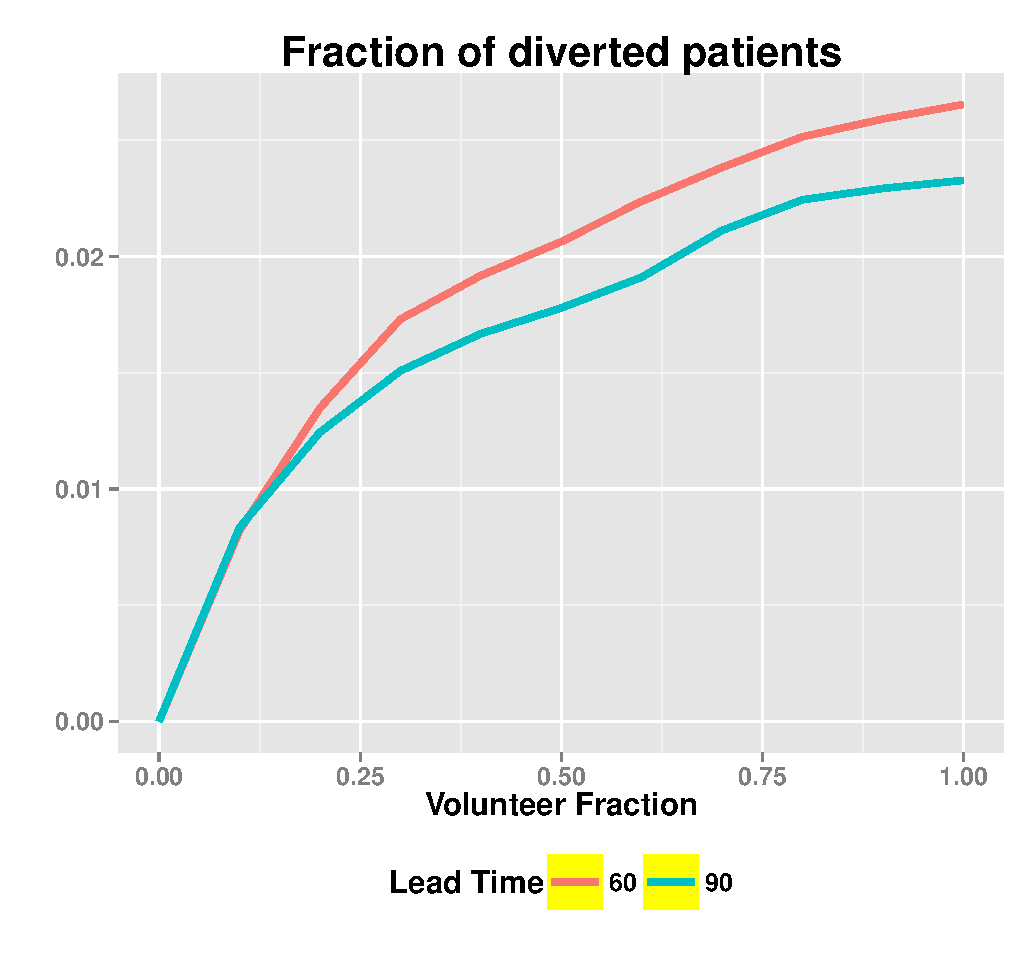
\includegraphics[width=.6\textwidth]{chap3/numeric/pic/3sites_diversion}
\caption{The fraction of patients diverted over all patients.
Only very small fraction of patients are diverted even with
all patients as volunteers.}
\label{fig:3sites_diversion}
\end{figure}

All of these are achieved with diverting
only at most 3\% of all patients as shown in Figure \ref{fig:3sites_diversion}.

\begin{figure}[htp]
\centering
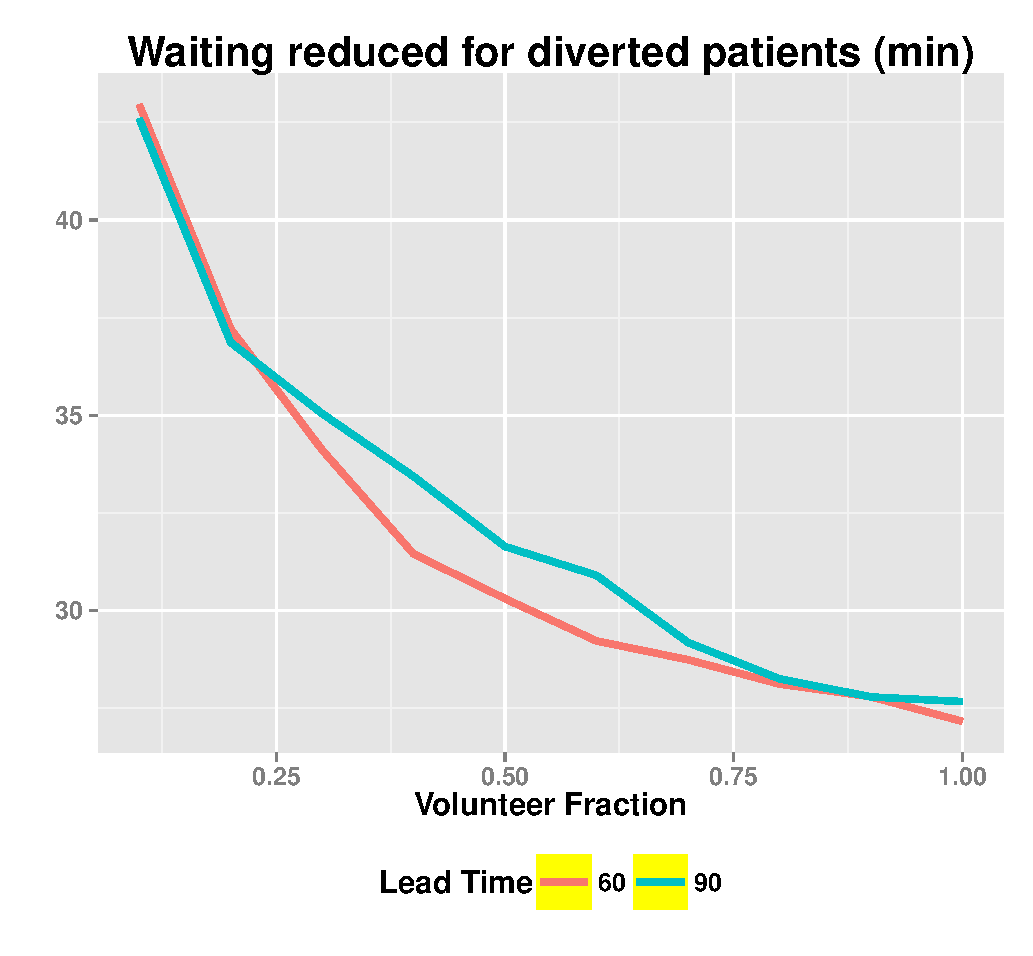
\includegraphics[width=.6\textwidth]{chap3/numeric/pic/3sites_gain}
\caption{Average waiting time reduced for diverted patients.
With more volunteers, the average gain decreases, but it's
still more than 25min with 100\% volunteers.}
\label{fig:3sites_gain}
\end{figure}

Figure \ref{fig:3sites_gain} shows how much waiting
time do the diverted patients save on average. Although it decreases
when we have more volunteers, but still there on average a diverted
patient is expected to wait at least 25min less, which is good incentive
for them to accept diversions. Another thing we can see is that
when we use 90min lead time, we can still achieve most benefits with
60min lead time. This shows that our approach is robust with longer
lead time.

\begin{figure}[htp]
\centering
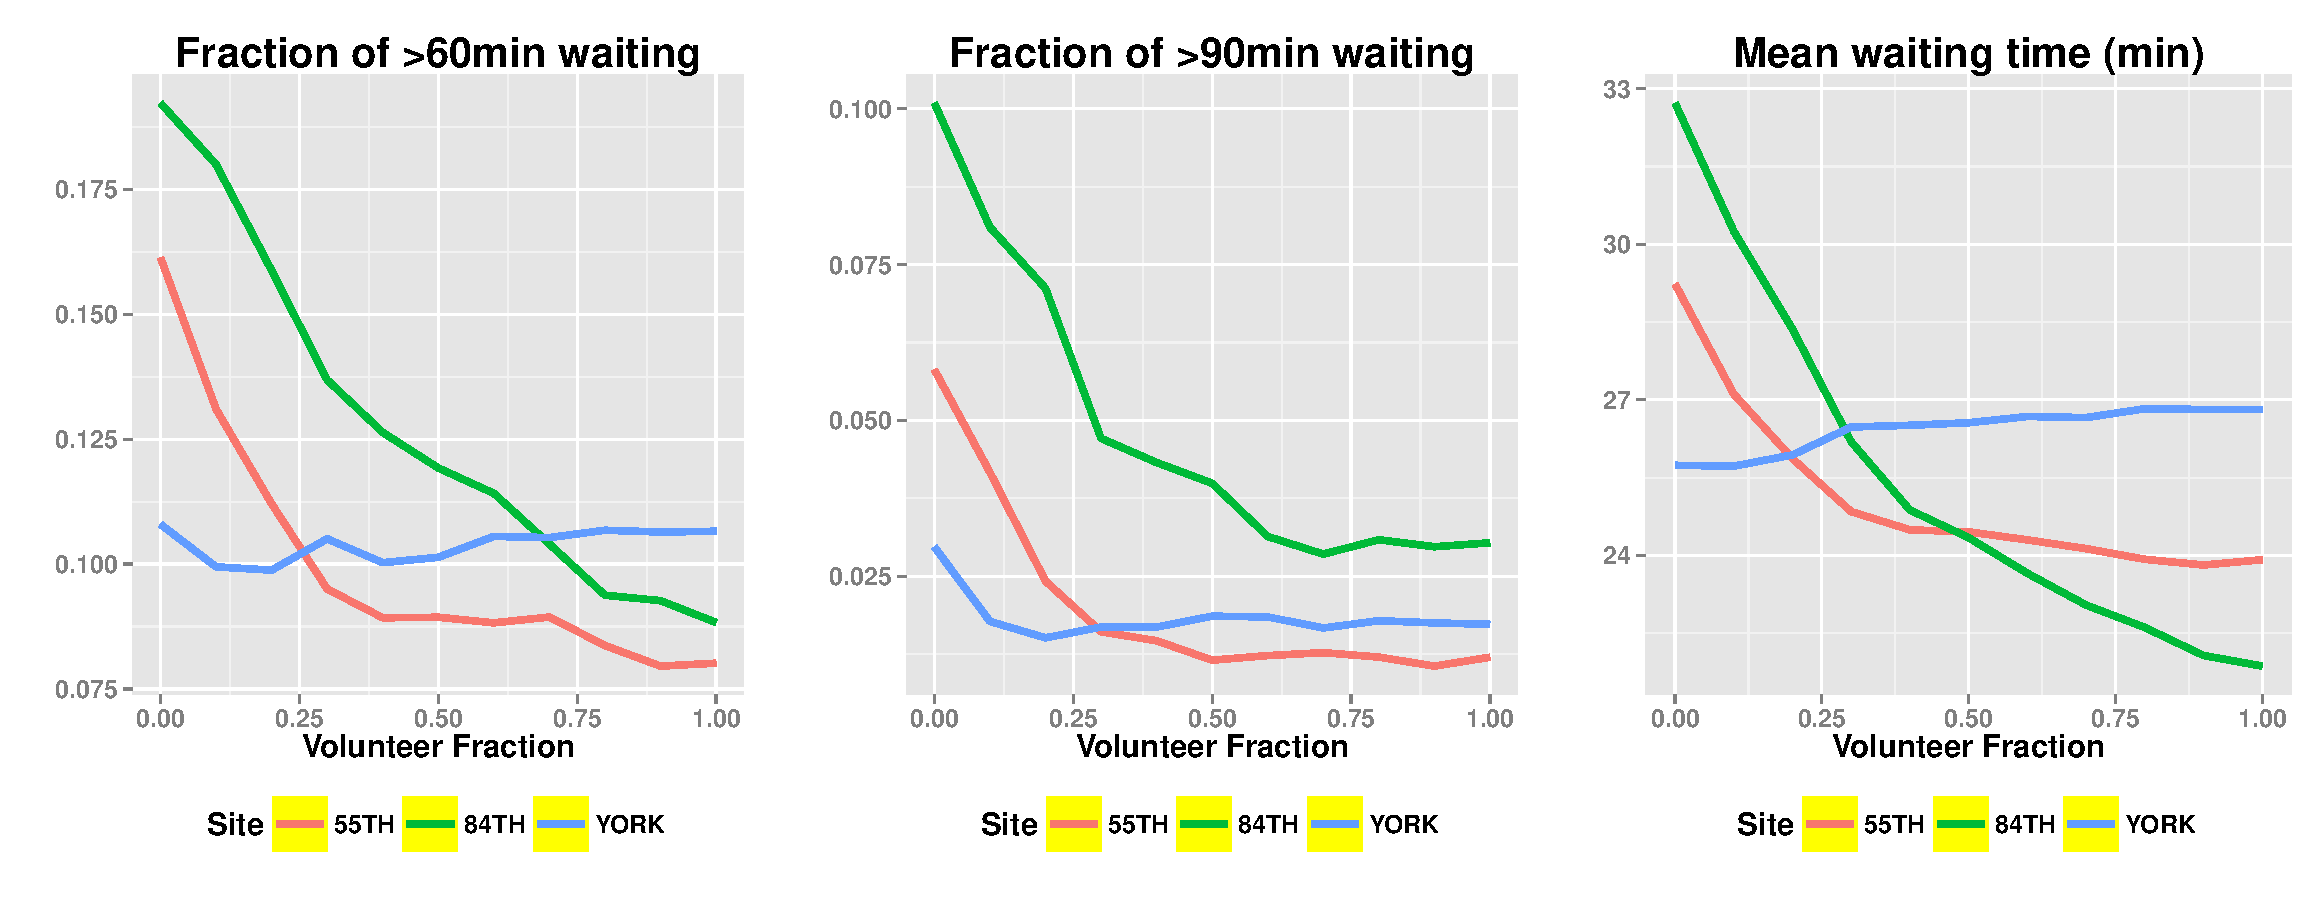
\includegraphics[width=.9\textwidth]{chap3/numeric/pic/3sites_site_wait}
\caption{Impact of diversions on waiting time for each site. It will
greatly improve situations at 55th St and West 84 St, but it will hurt
York Ave a little bit.}
\label{fig:3sites_site_wait}
\end{figure}

\begin{figure}[htp]
\centering
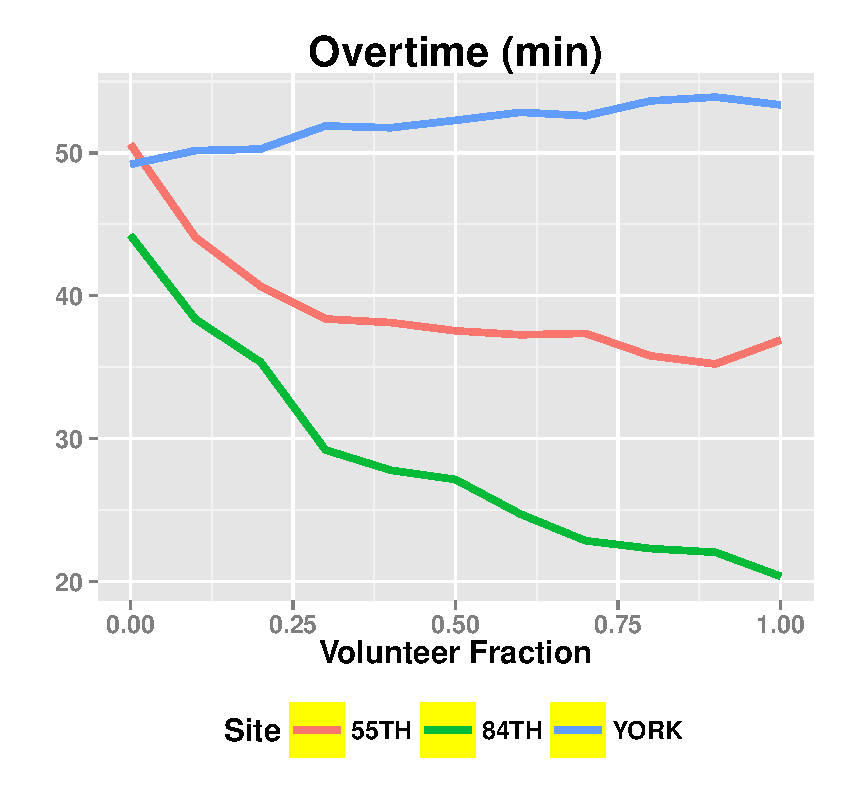
\includegraphics[width=.6\textwidth]{chap3/numeric/pic/3sites_site_overtime}
\caption{Impact of diversions on overtime for each site. Again it will hurt
York Ave a bit, but improves things at 55th St and West 84 St.}
\label{fig:3sites_site_overtime}
\end{figure}

It's also interesting to zoom in and look at what happens at site-level.
Figure \ref{fig:3sites_site_wait} shows the waiting time change per site. Here we see that
although the waiting time for 55th St and West 84th St improves a lot,
it becomes slightly worse. The same is true for overtime, as showed in
Figure \ref{fig:3sites_site_overtime}.

\begin{figure}[htp]
\centering
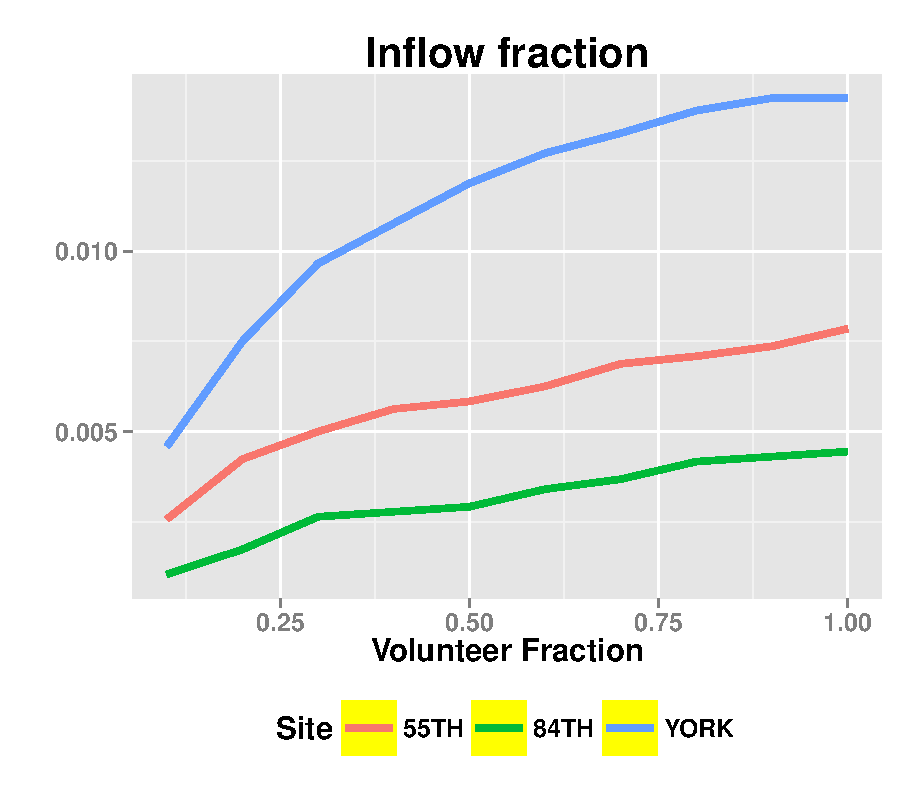
\includegraphics[width=.6\textwidth]{chap3/numeric/pic/3sites_site_inflow}
\caption{Fraction of patients diverted into each site. With four machines,
York Ave becomes the most popular destination and this explains why its
performance got hurt a bit.}
\label{fig:3sites_site_inflow}
\end{figure}

It becomes clear why when we look at Figure
\ref{fig:3sites_site_inflow}. It shows that among all diversions, most are inflow to York Ave.
The reason is that York Ave has 4 machines, so it already gets quite a
bit pooling and thus we're more likely to divert patients there.
However, as we see earlier, the overall performance of the whole
system still improves.

We also did experiment without disruptions like SDAOP or cancellation.
In this case, the system loads are lighter and the system is already
working quite well without diversion. But still, diversions can
produce some small improvement. See Figure \ref{fig:3sites_without_sdaop}.

\begin{figure}[htp]
\centering
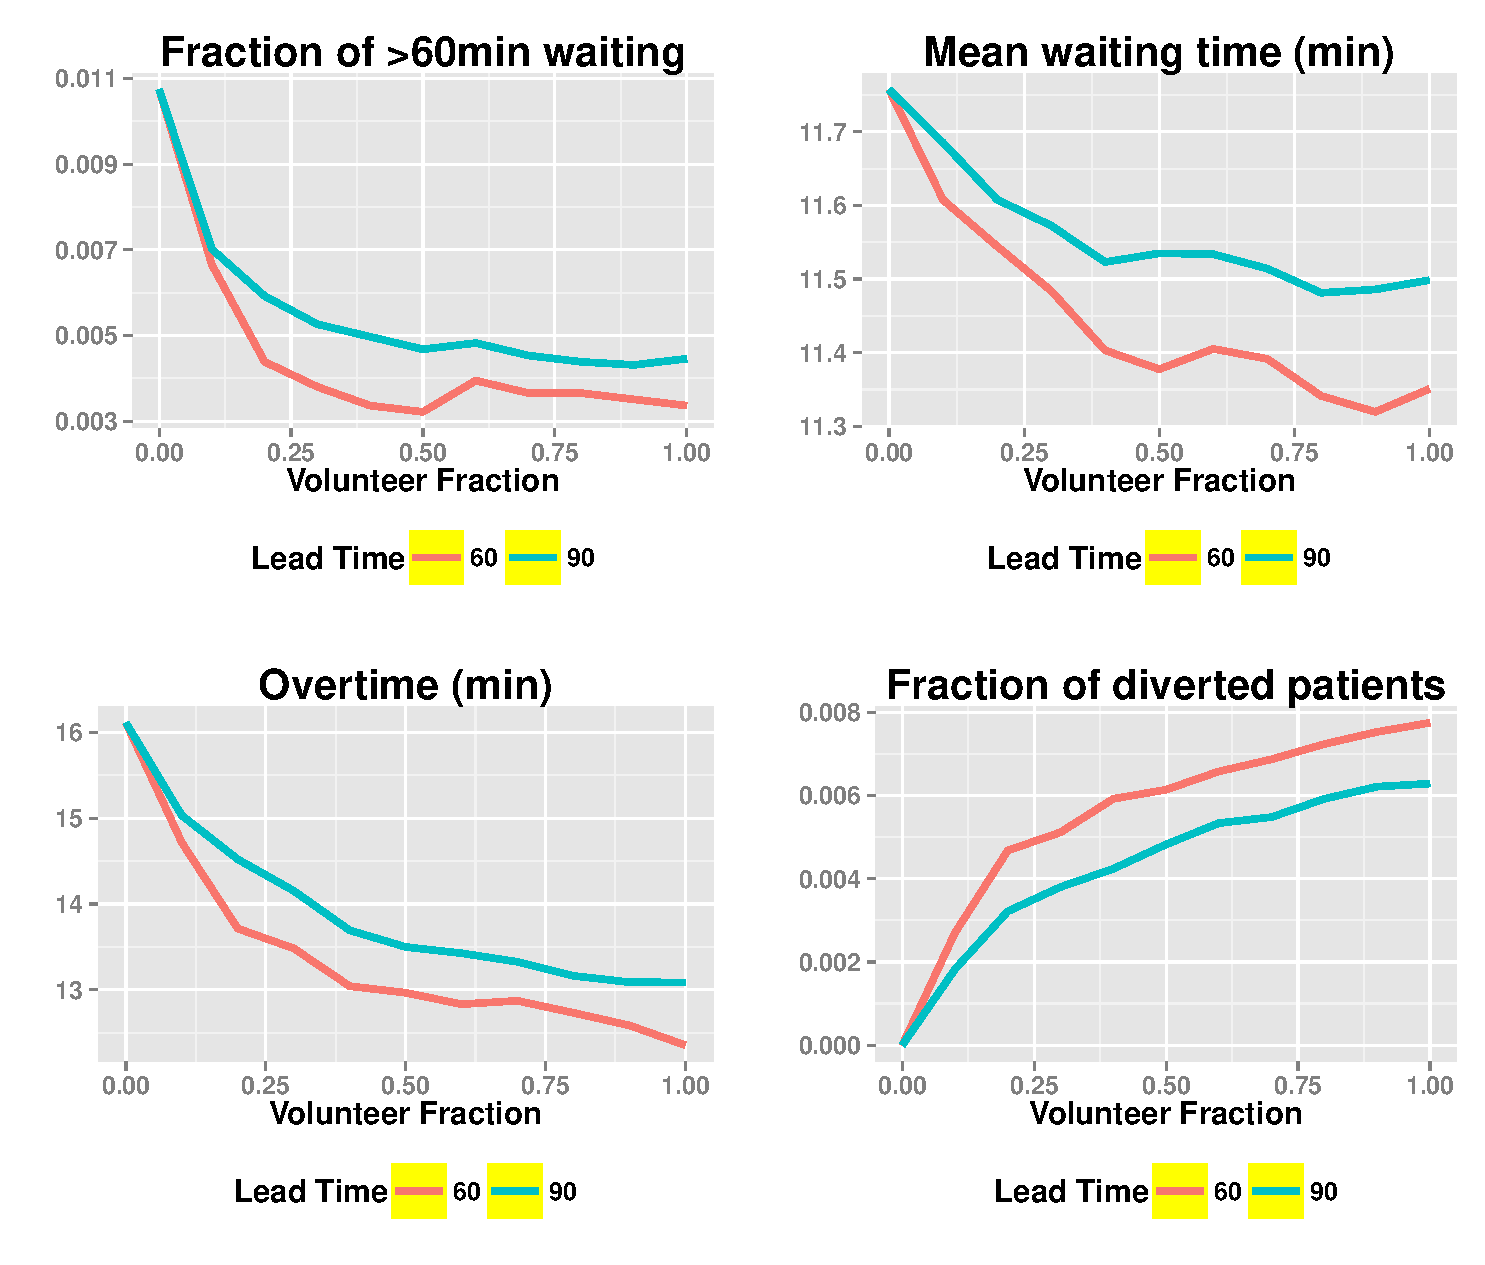
\includegraphics[width=.9\textwidth]{chap3/numeric/pic/3sites_without_sdaop}
\caption{System performance when there is no SDAOP and cancellation.
In this case, the system load is light and there isn't much congestion
to begin with. However, diversions can still achieve some small improvement.}
\label{fig:3sites_without_sdaop}
\end{figure}
